
\section{Model definition} % (fold)
\label{sec:model_definition}
	We introduce now the mathematical model used to represent our puzzle test-case system. As told earlier, we use a chemical reaction network framework (see Section~\ref{sec:chemical_reaction_networks} for background on this subject).

	We only consider the robot transporters scenario, the other scenario can be modeled in the same fashion.
	
	We assign a reaction to each assembly step in the creation of the final puzzles. Looking back at Figure~\ref{fig:assembly_plans}, each numbered assembly step corresponds to a reaction in our chemical reaction network.
	Furthermore, we add 4 new reactions, representing the grabbing of lying pieces by the robots.
	The products and reactants are the different mid-assemblies, plus the 3 lying free pieces and the robots. All reactions are second-order reactions, as they depend on the encountering of two different reactants upon reaction.
	
	We obtain the following chemical reaction network (Equation~\eqref{eq:reaction_network_transportersimple}):
	
	\begin{eqnarray}
		X_R + X_1^f ~~\xrightarrow{e_1} ~~ X_1 & \quad  & X_R + X_3^f ~~\xrightarrow{e_3} ~~ X_3 \nonumber \\
		X_R + X_2^f ~~\xrightarrow{e_2} ~~ X_2 & & X_R + X_4^f ~~\xrightarrow{e_4} ~~ X_4 \nonumber \\
		X_1 + X_2 ~~\xrightarrow{k_1} ~~ X_5 + X_R &  &  X_2 + X_7 ~~ \xrightarrow{k_4} ~~ X_{F1} + X_R\nonumber \\
		X_3 + X_4 ~~\xrightarrow{k_2} ~~ X_6 + X_R& & X_2 + X_5	~~ \xrightarrow{k_5} ~~ X_{8} + X_R \nonumber \\
		X_5 + X_6 ~~\xrightarrow{k_3} ~~ X_7 + X_R & & X_6 + X_8 ~~ \xrightarrow{k_6} ~~ X_{F2} + X_R
	\label{eq:reaction_network_transportersimple}
	\end{eqnarray}
	
	$X_R$ is a robot, $X_i^f$ are the free lying pieces, $X_k$ are the carried pieces and $X_{Fj}$ the final puzzles.
	
	The variables can be defined as the number of each piece type, where the number is a continuous function of time~\cite{Gillespie:1977p5555}. This network can then be transformed in the following associated ODE system (Equation~\eqref{eq:ode_transportersimple}):
	
	\begin{equation}
		\left\lbrace\begin{array}{lll}
			\dot{x_R} & = & -\sum_{l=1}^4 e_lx_Rx_l^f + k_1x_1x_2 + k_2x_3x_4 +  \\
			& & \qquad k_3x_5x_6 + k_4 x_2 x_7 + k_5 x_2 x_5 + k_6 x_6 x_8 \\
			\dot{x_1^f} & = & -e_1x_Rx_1^f \\
			\dot{x_2^f} & = & -e_2x_Rx_2^f \\
			\dot{x_3^f} & = & -e_3x_Rx_3^f \\
			\dot{x_4^f} & = & -e_4x_Rx_4^f \\
			\dot{x_1} & = & e_1x_Rx_1^f -k_1x_1x_2 \\
			\dot{x_2} & = & e_2x_Rx_2^f -k_1x_1x_2 -k_4x_2x_7 -k_5x_2x_5\\
			\dot{x_3} & = & e_3x_Rx_3^f -k_2x_3x_4 \\
			\dot{x_4} & = & e_4x_Rx_4^f -k_2x_3x_4 \\
			\dot{x_5} & = & k_1x_1x_2 -k_3x_5x_6 - k_5x_2x_5  \\
			\dot{x_6} & = & k_2x_3x_4 -k_3x_5x_6 - k_6x_6x_8 \\
			\dot{x_7} & = & k_3 x_5 x_6 -k_4 x_2 x_7 \\
			\dot{x_8} & = & k_5 x_2 x_5 -k_6x_6x_8 \\
			\dot{x}_{F1} & = & k_4x_2x_7 \\
			\dot{x}_{F2} & = & k_6x_6x_8 
		\end{array}\right.
		\label{eq:ode_transportersimple}
	\end{equation}
	
	Obviously, this notation is less compact, yet has the same meaning.
	
	We can also represent the network in matrix form:
	
	\[
		\mathbf{\dot{x}} = \mathbf{S} \mathbf{K} \mathbf{y}
	\]
	$\mathbf{S}$ is the stoichiometric matrix, containing the stoichiometric coefficients $m_r$ and $n_p$ as defined in Equation~\eqref{eq:general_chemical_reaction} in Section~\ref{sub:theory}. $\mathbf{K}$ is the matrix of stochastic constant rates. $y$ is a vector of compounds, in our case the set of all bilinear terms in Equation~\eqref{eq:ode_transportersimple} for example.
	
	We can also relax the $x_R$ and $x_i^f$ terms, if we decide to look only at the real assembly process therein. Doing so is consistent if we assume that we have a big number of robots to carry the pieces around, and that they grab the pieces very quickly compared to the actual assembly process. This approach is similar as doing a quasi-steady state simplification, for a multiscale system where the robots are acting quicker than the rest of the system. Such a relaxation simplifies the whole system and its analysis, we will use it in the next chapter.
% section model_definition (end)

	\subsection{Simulation of the model} % (fold)
	\label{sub:simulation_of_the_model}
		We simulate our models using two different approaches:
		\begin{enumerate}
			\item ODE solving. We use Matlab to solve numerically the system \eqref{eq:ode_transportersimple}, using a classical ode45. We use libSBML~\cite{Bornstein:2008p7529} for Matlab to write and read from SBML files onto ODE files.
			\item Stochastic Simulation Algorithm. We use the StochKit toolbox~\cite{Li:2008p11431}, developed by Petzold et al. StochKit is a simulation framework for stochastic simulations written in C++. It allows a very fast exact simulations of chemical reaction networks.
		\end{enumerate}
	% subsection simulation_of_the_model (end)
	
\section{Parameter fitting} % (fold)
\label{sec:parameter_fitting}
	
	\subsection{Theoretical value of reaction rates} % (fold)
	\label{sub:theoretical_value_of_reaction_rates}
	
		The chemical reaction network is easy constructed from the assembly plans considered, but we still need to find values for the stochastic constant rates~$k_i$ and~$e_l$.
	
		We decompose the stochastic constant rates as follows:
	
		\begin{equation}\label{eq:reaction_assembly_rate}
			k_i = p^e_i \cdot p^a_i
		\end{equation}
	
		where $p^e_i$ is the probability of an encounter between two elements and $p_i^a$ the probability of successful assembly.
	
		$p_i^a$ can be easily measured, or assumed to be $1$ if the robots manage to align the pieces correctly before each assembly step.
	
		If we assume that our model is non-spatial, i.e. that the probability that two product are at a given position is independent of the time and uniformly distributed over the available arena space, we can make an initial informed guess on the encountering probability. We take an approach used in~\cite{Correll:2007p8184, Correll:2007p8236, Correll:2006p8328}, giving the following relation for the encountering probability:
	
		\begin{equation} \label{eq:encountering_probability}
			p^e_i \sim \frac{1}{A_{total}}v_rTw_d^i
		\end{equation} 
	
		Where $A_{total}$ is the arena size, $v_r$ is the average speed of an element, $T$ is the timestep (fixed to $1$ in our case) and $w_d^i$ the width of detection of an element. This expression can actually be linked back to the literature on chemical process simulations~\cite{Gillespie:1992p8126, Puchalka:2004p4312, Turner:2004p4446}. For chemical process, the probability of collision depends on the volume swept by one molecule, which gives the probability that another molecule will collide it in the next $dt$. Equation~\eqref{eq:encountering_probability} is exactly the same, as shown on Figure~\ref{fig:volume_swept}. In our case, as we work in a 2D plan, we only have surface swept, which is exactly given by the right part of \eqref{eq:encountering_probability}. Dividing by the total arena size and assuming the elements are distributed uniformly in the arena, this gives directly the probability of encountering between two elements.
	
		\begin{figure}[h]
			\centering
			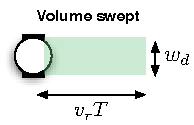
\includegraphics[width=4cm]{img/volume_swept.pdf}
			\caption{Graphical interpretation of the encountering probability and link to the volume swept used in chemical simulations.}
			\label{fig:volume_swept}
		\end{figure}
	
		In our test case, we measured $v_r$ over 50 simulation runs using the robot movement pattern described earlier, the average speed was $0.128 m/s$. $A_{total}$ is also easily computed ($=6 (R^2\frac{\sqrt{3}}{4})$, i.e. the sum of the six equilateral triangles of radius $R$). $w_d^i$ becomes the double of the communication radius between robots or pieces, as it defines the range for the start of an assembly.
	
	% subsection theoretical_value_of_reaction_rates (end)
	
	\subsubsection{Rates verification} % (fold)
	\label{ssub:rates_verification}
		We checked this initial guess by measuring the encountering rates in Webots. We create a world with one lying piece and one searching robot, we measure the time to encounter, over 200 experiments. As discussed in the theory of chemical reaction networks, these times are distributed following an exponential of the encountering probability. We load the times in Matlab, and fit an exponential distribution to get this probability (Figure~\ref{fig:img_encountering_exp_fitting}).
		\begin{figure}[h]
			\centering
				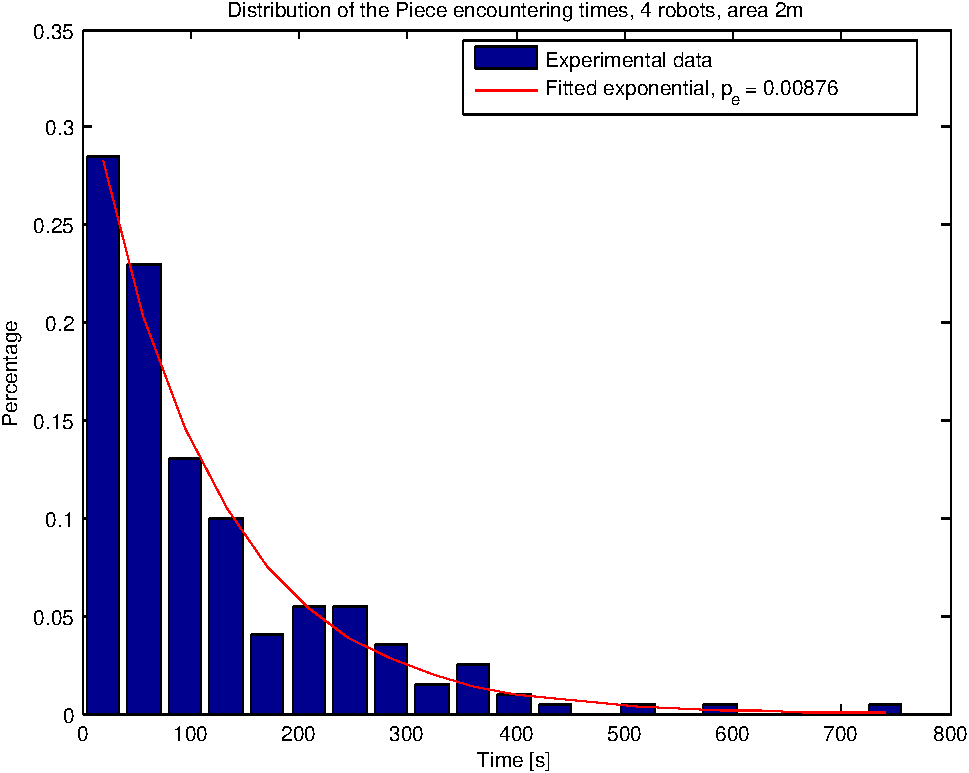
\includegraphics[width=9cm]{img/encountering_exp_fitting.pdf}
			\caption{Encountering times for the Webots experiment, with the fitted Matlab exponential.}
			\label{fig:img_encountering_exp_fitting}
		\end{figure}
		
		We also add ``dummy'' robots in the arena, that only avoid each other without looking for the piece. It measures the effect of overcrowding on the well-mixed property we're trying to ensure within our Webots simulation.
		
		\begin{figure}[h]
			\centering
				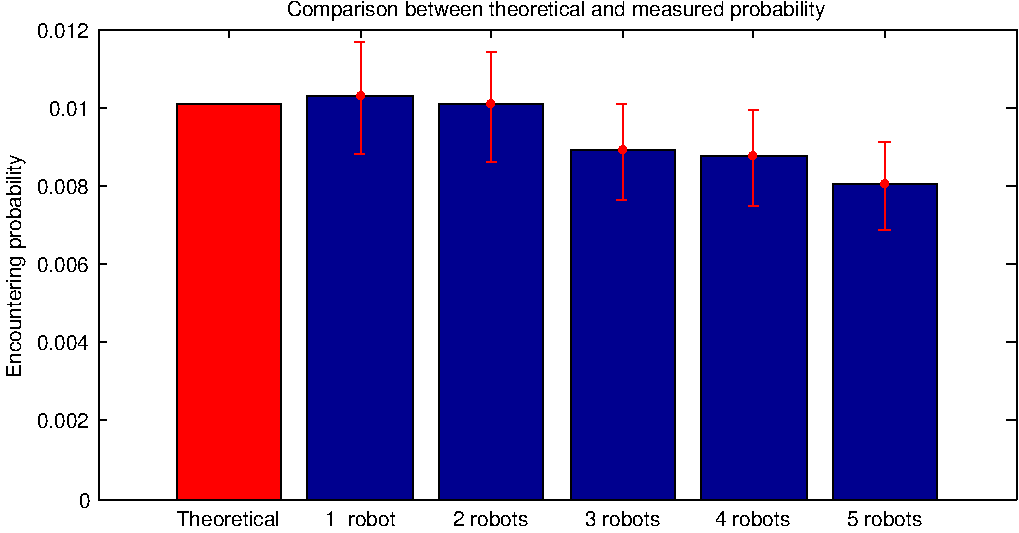
\includegraphics[width=11cm]{img/encounteringrate_withrobots.pdf}
			\caption{Comparison between the theoretical guess for the encountering probability $p_e^i$ and the measured encountering probability in Webots. The red intervals represents the confidence intervals for the fitted encountering probability.}
			\label{fig:img_encounteringrate_withrobots}
		\end{figure}
		
		The results of the comparison between the theoretical and measured rates of encountering are shown in Figure~\ref{fig:img_encounteringrate_withrobots}. We see that the theoretical guess is pretty accurate, even tough it is overestimated when more robots are present. The added robots seems to disturb the capacity of a robot to encounter a piece. This can be due to the fact that the robots perturbs the trajectories while avoiding each others, overcrowding some areas and forbidding the access to others.
		
		The same measurement was performed for robot to robot encountering and gave similar results. We do not show it here.
		
	% subsubsection rates_verification (end)	
% section parameter_fitting (end)

\section{Comparison with physical simulation} % (fold)
\label{sec:comparison_with_physical_simulation}
	
	We simulate the chemical reaction network \eqref{eq:reaction_network_transportersimple} using the two approaches presented in Section~\ref{sub:simulation_of_the_model}. Depending on the initial conditions for the number of robots and pieces, we have different experiments, following Section~\ref{sec:the_robot_transporters_scenario}.
	
	\subsubsection{Stochastic constant rates values} % (fold)
	\label{ssub:stochastic_constant_rates_values}
		Through all these experiments, the stochastic constant rates $e_l$ and $k_i$ take similar values, conditioned by specific parameters presented in each experiment setup.
		
		\begin{description}
			\item[Encountering rates] $e_l = \frac{1}{A_{total}}\cdot v_r \cdot w_d^p \quad \forall l \in \{1..4\}$.
			\item[Reaction rates] $k_i = p^a_i\cdot \frac{1}{A_{total}}\cdot v_r \cdot w_d^r \quad \forall i$.
			\item[Arena size] $A_{total}=3 \cdot R_a^2 \cdot \frac{\sqrt{3}}{2}$.
			\item[Average speed] $v_r = 0.128$ measured in Webots.
			\item[Piece communication width] $w_d^p = 2\cdot0.4m$, pieces are set to communicate in a $40cm$ radius.
			\item[Robot communication width] $w_d^r = 2\cdot0.6m$, robots are set to communicate in a $60cm$ radius.
			\item[Probability of successful assembly] $p^a_i$ depends on the experiment being studied, more precisely on the assembly plan used. We measured it in Webots, over 100 runs, for the assembly plan creating only the final puzzle F1 and for the assembly plan creating the final puzzles F1 and F2. Results will be specified in the experiments' setup.
		\end{description}
	
	% subsubsection stochastic_constant_rates_values (end)
	
	\subsection{Experiment 1: 5 pieces and 5 robots, final puzzle F1 only} % (fold)
	\label{sub:experiment_1_5_pieces_and_5_robots_final_puzzle_f1_only}
		Setup:
		\begin{description}
			\item[Initial conditions:] $X_R = 5, X_1^f=1, X_2^f=2, X_3^f=1, X_4^f=1, X_i=0, X_{Fk}=0$.
			\item[Experiment duration:] 20 minutes.
			\item[Number of experiments (Stochastic simulation only):] 100.
			\item[Arena size:] $R_a = 2m$.
			\item[Probability of successful assembly:] all $p^a_i$ where more or less equal to $0.98$. Thus we set $p^a_i = 0.98$.
		\end{description}
				
		See Figure~\ref{fig:models_comparison_experiment1} for the comparison between the simulated chemical reaction networks and the Webots physical simulation. The results from the Webots simulation are taken from Section~\ref{ssub:experiment_1_5_pieces_and_4_robots}. We show the averaged populations over 20 minutes.
				
		\begin{figure}[h!]
			%\centering
			\subfigure[ODE simulation vs physical Webots simulation] 
			{
				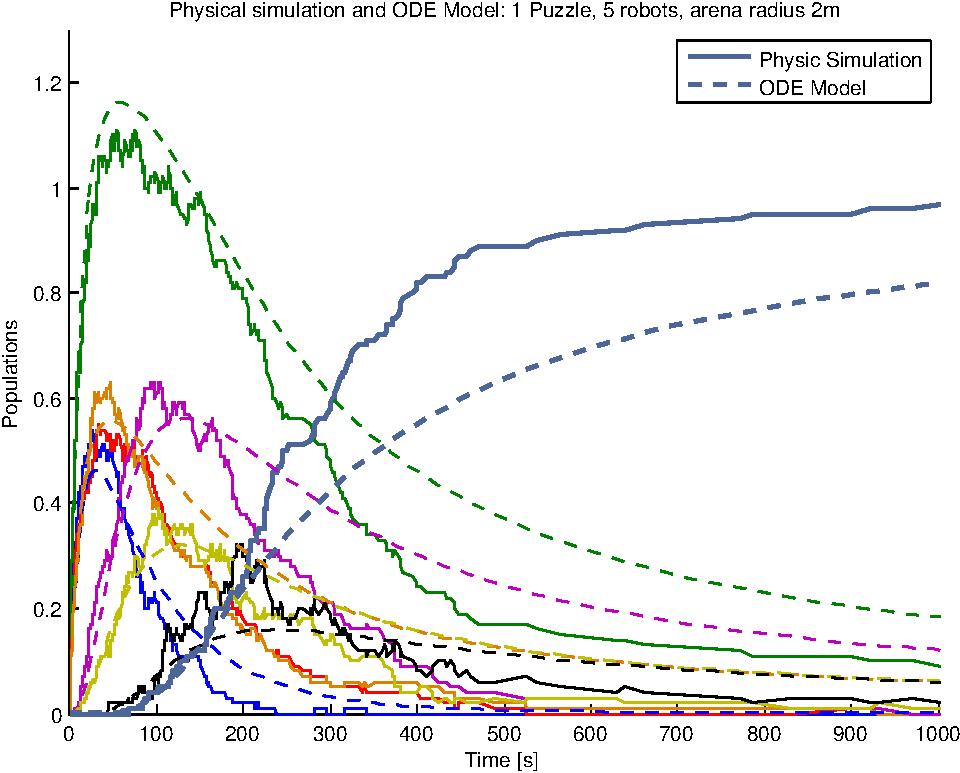
\includegraphics[width=7cm]{img/odereal_1puzzle.pdf}
				\label{fig:models_comparison_experiment1:odereal}
		 	}
			\: % espacement entre figures. \quad \;
			\subfigure[Stochastic simulation vs physical Webots simulation] 
			{
				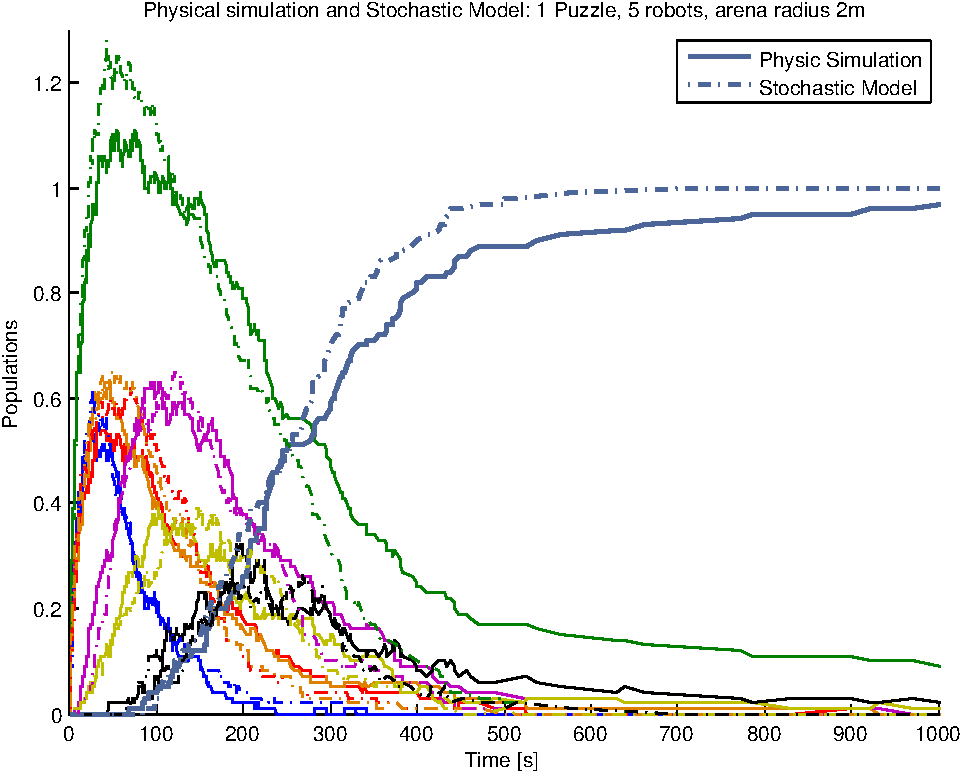
\includegraphics[width=7cm]{img/stochreal_1puzzle.pdf}
				\label{fig:models_comparison_experiment1:stochreal}
		 	}
			\caption{Comparison between the models simulations and the physical Webots simulation for the puzzle test-case, scenario 1, experiment 1.}
		\label{fig:models_comparison_experiment1} %Caption general
		\end{figure}
			
		We see that they fit closely to the physical simulation. Two differences arise:
		
		\begin{my_itemize}
			\item The ODE simulation population values are too small, because of the slow copy number of components (Figure~\ref{fig:models_comparison_experiment1:odereal}). When doing an ODE approximation, one assumes that the number of components is big enough so that using continuous numbers does not have much effects. This is not the case here, where we work with numbers smaller than $10$. On the other hand, the Stochastic simulation accurately captures this property, as it works with discrete numbers. 
			\item The stochastic simulation attains 1, whereas the physical simulation stays below (Figure~\ref{fig:models_comparison_experiment1:stochreal}). These results show that, while there are problems in the Webots simulation (pieces stuck together, blocked against the walls), this is not taken into account in the model. We could modify the model by introducing ways of deactivating some pieces to try to fit this difference. But we do not take much interest in that for this current work.
		\end{my_itemize}
		
	% subsection experiment_1_5_pieces_and_5_robots_final_puzzle_f1_only (end)
	
	\subsection{Experiment 2: 15 pieces and 15 robots, final puzzle F1 only} % (fold)
	\label{sub:experiment_2_15_pieces_and_15_robots_final_puzzle_f1_only} 
		Setup:
		\begin{description}
			\item[Initial conditions:] $X_R = 15, X_1^f=3, X_2^f=6, X_3^f=3, X_4^f=3, X_i=0, X_{Fk}=0$.
			\item[Experiment duration:] 20 minutes.
			\item[Number of experiments (Stochastic simulation only):] 100.
			\item[Arena size:] $R_a = 3m$.
			\item[Probability of successful assembly:] $p^a_i = 0.98$.
		\end{description}
			
		Under the same assumptions than for experiment 1, see Figure~\ref{fig:models_comparison_experiment2} for the comparison in this scenario.			
			
		\begin{figure}[h!]
			%\centering
			\subfigure[ODE simulation vs physical Webots simulation] 
			{
				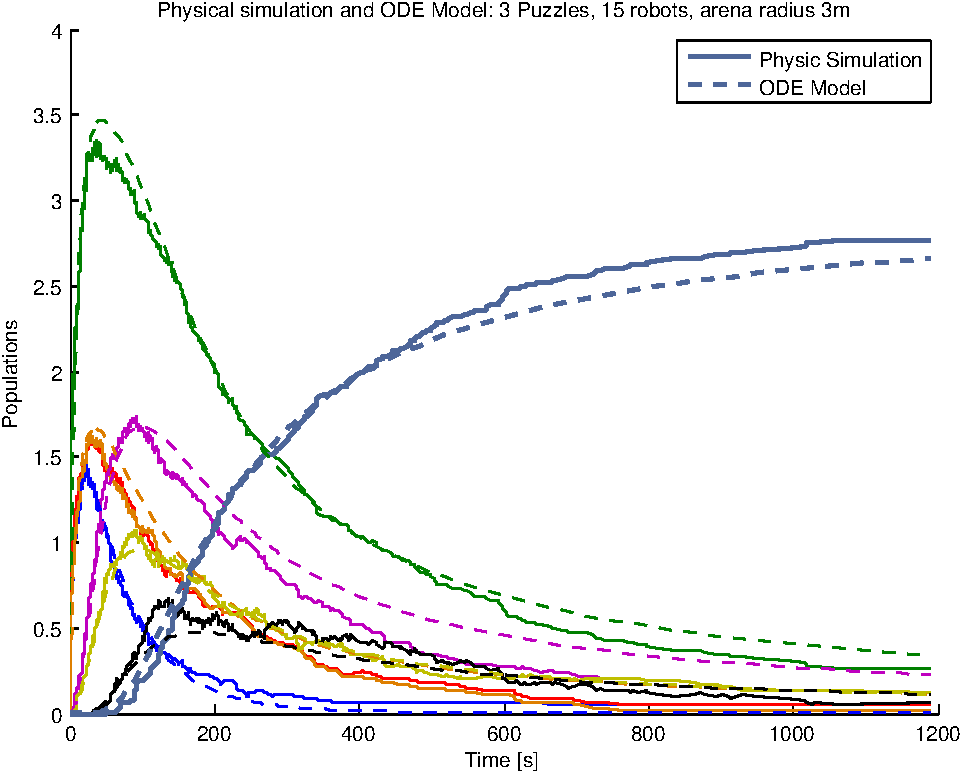
\includegraphics[width=7cm]{img/odereal_3puzzle.pdf}
				\label{fig:models_comparison_experiment2:odereal}
		 	}
			\: % espacement entre figures. \quad \;
			\subfigure[Stochastic simulation vs physical Webots simulation] 
			{
				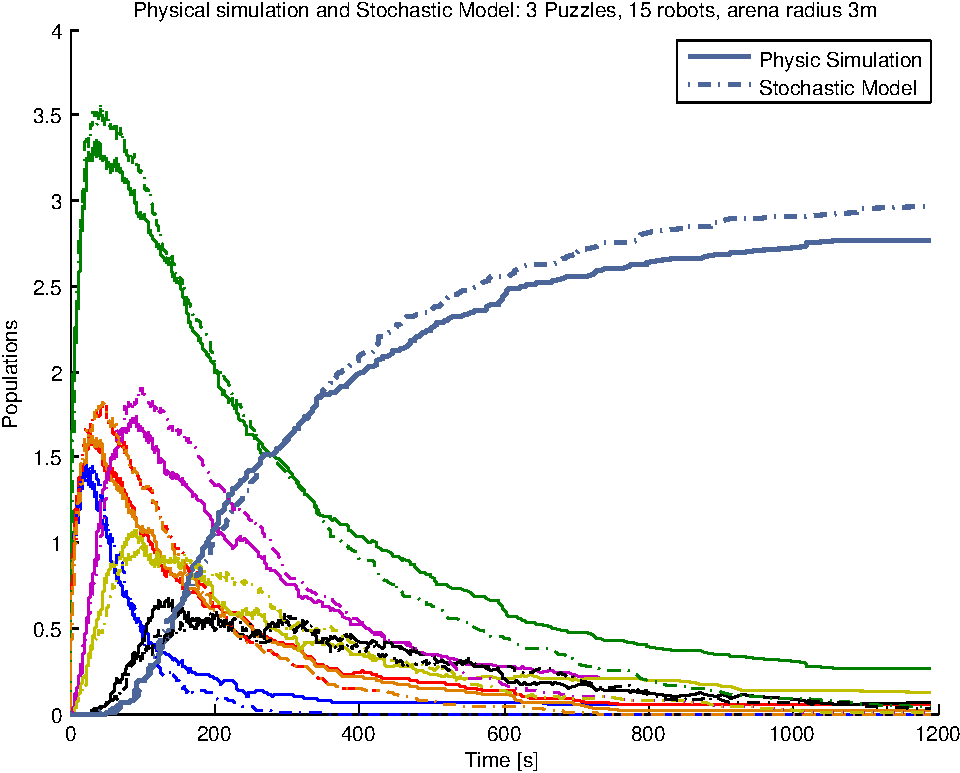
\includegraphics[width=7cm]{img/stochreal_3puzzle.pdf}
				\label{fig:models_comparison_experiment2:stochreal}
		 	}
			\caption{Comparison between the models simulations and the physical Webots simulation for the puzzle test-case, scenario 1, experiment 2.}
		\label{fig:models_comparison_experiment2} %Caption general
		\end{figure}
			
		The results are similar to experiment 1. With a higher number of elements, the ODE simulation is closer to the correct physical simulation. The stochastic simulation is still very accurate but attains the maximal number of puzzles whereas the physical simulation converge to a lower value.
		
	% subsection experiment_2_15_pieces_and_15_robots_final_puzzle_f1_only (end)
	
	\subsection{Experiment 3: 5 pieces and 5 robots, final puzzles F1 and F2} % (fold)
	\label{sub:experiment_3_5_pieces_and_5_robots_final_puzzles_f1_and_f2}
	
		Setup:
		\begin{description}
			\item[Initial conditions:] $X_R = 5, X_1^f=1, X_2^f=2, X_3^f=1, X_4^f=1, X_i=0, X_{Fk}=0$.
			\item[Experiment duration:] 20 minutes.
			\item[Number of experiments (Stochastic simulation only):] 100.
			\item[Arena size:] $R_a = 2m$.
			\item[Probability of successful assembly:] Results of the measures are shown in Table~\ref{tab:assembly_success_experiment3}. We see that now, the probabilities are not equal and depend on the assembly step. Especially, the success of reaction 5, to create piece 8, is significantly smaller. $p^a_i$ is set accordingly for each reaction $i$.
		\end{description}
				
		\begin{table}
			\begin{center}
			\begin{tabular}{|c|c|c|c|c|c|c|}
			 \hline
				\textbf{Reaction} $\mathbf{i}$ & 1 & 2 & 3 & 4 & 5 & 6 \\
			 \hline
				$\mathbf{p^a_i}$ & 0.9777 & 0.9074 & 0.9636 & 0.9737 & 0.833 & 1.0 \\
			 \hline
			\end{tabular}
			\end{center}
			\caption{Probability of successful assembly for experiment 3. Measured over 100 experiments.}
			\label{tab:assembly_success_experiment3}
		\end{table}
		
		See Figure~\ref{fig:models_comparison_experiment3} for the results.
		
		\begin{figure}[h!]
			%\centering
			\subfigure[ODE simulation vs physical Webots simulation] 
			{
				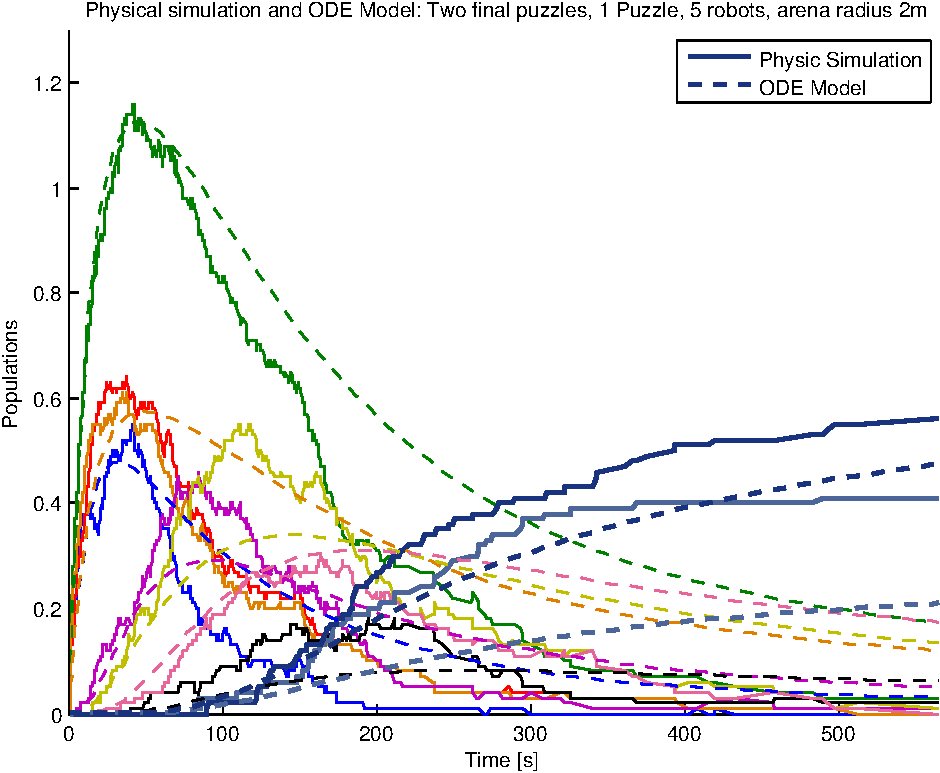
\includegraphics[width=7cm]{img/odereal_2finals_1puzzle.pdf}
				\label{fig:models_comparison_experiment3:odereal}
		 	}
			\: % espacement entre figures. \quad \;
			\subfigure[Stochastic simulation vs physical Webots simulation] 
			{
				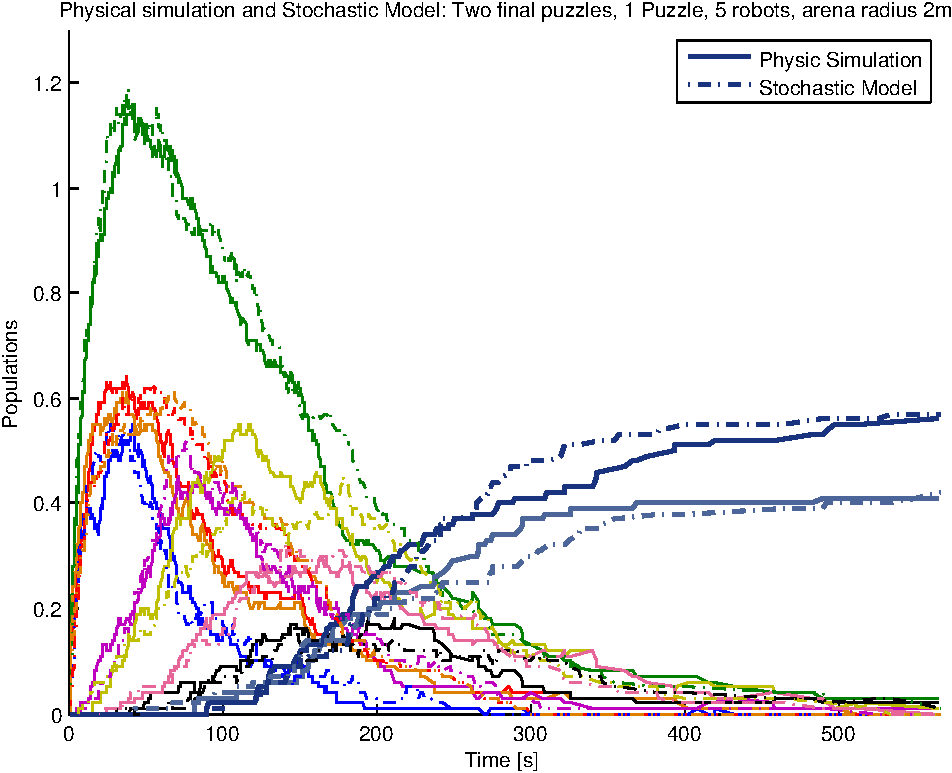
\includegraphics[width=7cm]{img/stochreal_2finals_1puzzle.pdf}
				\label{fig:models_comparison_experiment3:stochreal}
		 	}
			\caption{Comparison between the models simulations and the physical Webots simulation for the puzzle test-case, scenario 1, experiment 3.}
		\label{fig:models_comparison_experiment3} %Caption general
		\end{figure}
		
		We see that the ODE model fails to capture the time to convergence, and underestimates the speed of variations. It also seems that they do not converge to the same values, which could be a problem. However, using the Stochastic simulation with the exact same rates, we see that the fitting is much better. The low copy numbers again has a big impact on the capacity to use the ODE model as an approximation.
			
		But the rates we use for the ODE model produce a good fit when using the Stochastic simulation, which shows that our model accurately describes the physical system's dynamics. We thus think that, if the copy number is big enough, the analysis with the ODE model should be sufficient.
		
		We confirm this hypothesis by performing the same two final puzzles experiment, with 15 pieces and 15 robots and a bigger arena (like Experiment 2). The parameters are adapted accordingly. We obtain the results shown in Figure~\ref{fig:models_comparison_experiment3bis}.
		
		\begin{figure}[h!]
			%\centering
			\subfigure[ODE simulation vs physical Webots simulation] 
			{
				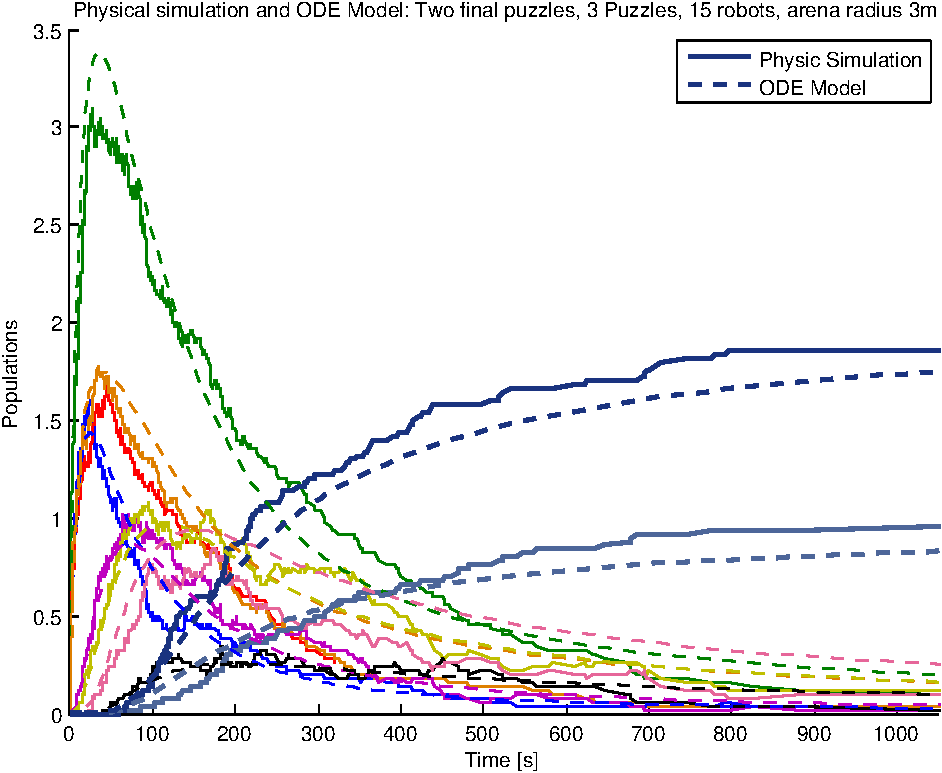
\includegraphics[width=7cm]{img/odereal_2finals_3puzzle.pdf}
				\label{fig:models_comparison_experiment3bis:odereal}
		 	}
			\: % espacement entre figures. \quad \;
			\subfigure[Stochastic simulation vs physical Webots simulation] 
			{
				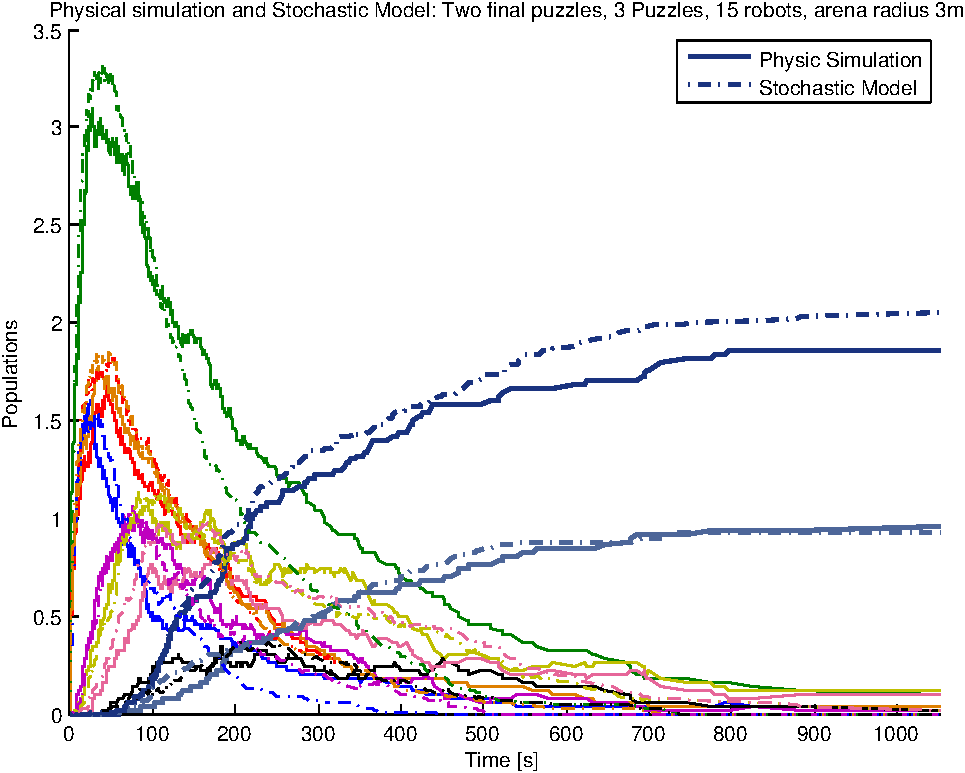
\includegraphics[width=7cm]{img/stochreal_2finals_3puzzle.pdf}
				\label{fig:models_comparison_experiment3bis:stochreal}
		 	}
			\caption{Modified experiment 3 with 15 pieces and 15 robots, to show the effect of a larger copy number.}
		\label{fig:models_comparison_experiment3bis} %Caption general
		\end{figure}
		
		This confirms our assumption that the only problem with the ODE model discrepancy of convergence is the low copy number. In this new scenario, the fitting of the ODE simulation is good and converge to the physical values (Figure~\ref{fig:models_comparison_experiment3bis:odereal}). This tells us that we can indeed use the ODE as a model, but only for a copy number large enough. We will take advantage of that fact in the next chapter.
		
		
	% subsection experiment_3_5_pieces_and_5_robots_final_puzzles_f1_and_f2 (end)
	
% section comparison_with_physical_simulation (end)

\section{Final considerations} % (fold)
\label{sec:final_considerations}
	
	The comparison between the models and the Webots physical simulations shows a close fit of our model to the experimental data. It proves that this model is accurate for our test-case and considered problem. The stochastic simulation captures the correct behavior when the number of elements is small, which is in accordance with the assumptions on algorithms differences.
	
	Therefore, we will use directly the model into an optimization process, before mapping back the new model onto the physical simulation. This approach makes sense, as thanks to the accuracy of our model, we can then hope that the physical simulation will behave in the same way. The only constraint is that we need to work with big copy numbers with the ODE, to avoid convergence problems.
	
	Some problems are still present.
	For example, the initial guess for the encountering probability becomes wrong when the number of robots and pieces grows. The guess relies on a strong non-spatiality constraint, which our physical simulation can not ensure in several cases. Our models do not capture the failures of the physical simulations, which hinder the overall performance and reliability of the assembly process. 
% section final_considerations (end)